% =====================================================================
% DocStruct --- draft 5, 2026-09-03. Narrative rewrite on the ACL 2023 template.
%
% Compile: pdflatex main && bibtex main && pdflatex main && pdflatex main
%
% Every number in this file resolves to a row in
% .claude/skills/acl-paper/references/claim-ledger.md, which names the report
% that produced it. Every OHR-Bench number names its relevance rule.
%
% Withdrawn numbers that must NEVER reappear (notes.md 2026-08-16): the internal
% arXiv five-tool table, the ablation deltas +0.0429 / +0.0138 / -0.0101, the
% vision detector's +0.0443, and coverage 0.817 / duplication 2.06.
%
% Camera-ready: restore the repository URL in the footnote of Section 1
% (https://github.com/CandyButcher27/DocStruct) and fill the author block.
% =====================================================================
\pdfoutput=1
\documentclass[11pt]{article}

\usepackage[review]{ACL2023}

\usepackage{times}
\usepackage{latexsym}
\usepackage[T1]{fontenc}
\usepackage[utf8]{inputenc}
\usepackage{microtype}
\usepackage{inconsolata}

\usepackage{booktabs}
\usepackage[font=small,skip=3pt]{caption}
\usepackage{graphicx}
\graphicspath{{figures/}}
\usepackage{amsmath}
\usepackage{amssymb}
\usepackage{xcolor}
\usepackage{tikz}
\usetikzlibrary{arrows.meta, fit, positioning}

\newcommand{\ds}{\textsc{DocStruct}}
\newcommand{\dsg}{\textsc{DocStruct}-\textsc{geo}}
\newcommand{\best}[1]{\textbf{#1}}

\title{\ds{}: Layout-Aware {PDF} Chunking for Structured Document Retrieval}

\author{
 Aryaman Srivastava \\
  \texttt{srivastavaaryaman555@gmail.com}
  % TODO before camera-ready: affiliation and co-authors.
}

\begin{document}
\maketitle

\begin{abstract}
PDF documents encode information through both text and spatial layout, but conventional extraction loses the layout before the text reaches a retrieval system: columns interleave, tables fragment, and sections mix during chunking. We present \ds{}, a deterministic chunking engine that recovers layout first. A geometry-based detector finds structural blocks, an optional vision model proposes blocks in parallel, and the fused blocks are ordered and used to rebuild the heading hierarchy before any chunk is cut. No language model runs on this path, so the same PDF always yields the same chunks. Against five existing chunkers and a geometry-only variant of our own, on 3{,}558 human-written questions, \ds{} ranks first under two relevance rules and sixth under a third, on identical chunks. It also returns about four times more context per query than the leanest baseline, which the first two rules reward, and the vision model adds no measurable retrieval gain.
\end{abstract}

% =====================================================================
\section{Introduction}
\label{sec:intro}

When we open an academic paper in a PDF viewer, we can view its two columns neatly and in the intended reading order. However, when the same paper is processed by a conventional text extractor, the extracted text may interleave the columns: the first line of the left column may be followed by the first line of the right column, followed by the second line of the left column. The PDF contains the positions of the characters and other graphical elements, but the semantic structure of the page, such as which text belongs to a column, heading, table, or caption, must be inferred from this layout. If an extraction pipeline does not perform this inference, it can traverse the text in an order that differs from how a reader would naturally read the document. By the time the resulting text is passed to a chunker that splits it by character count or nearby blank lines, much of the original layout information has already been lost.

There are two broad approaches to this problem. The first is to accept this loss of structure and use simple, cheap, and repeatable splitting methods. The second is to introduce contextual methods that determine where topics or semantic boundaries change, such as language-model-based approaches \citep{duarte2024lumberchunker}, or methods that cluster sentence embeddings based on semantic similarity \citep{smith2024chunking}. The first approach can lose information because it does not account for the natural flow of the document and may split sentences, paragraphs, or related ideas across different chunks. The second approach provides greater contextual awareness, but introduces additional computational and operational costs. It may require external model calls, tie the pipeline to a particular model or version, and introduce variability in the resulting chunks.

\ds{} takes a third approach by recovering document structure before performing chunking. In born-digital PDFs, much of the information needed to reconstruct this structure is available through the document geometry, including font properties, ruling lines, whitespace, and the positions of text elements. \ds{} uses geometry-based methods to identify blocks on each page and can optionally incorporate proposals from a vision model. These signals are then reconciled before the blocks are arranged into a reader-oriented order. The pipeline subsequently extracts text and tables, reconstructs the document's heading hierarchy, and generates chunks only after this structure has been established (Figure~\ref{fig:pipeline}). Each resulting chunk retains information about its page, position in reading order, block type, and associated headings.

Keeping language models off the parsing path makes the pipeline deterministic, and its core needs no network or GPU.

We evaluate \ds{} using three relevance criteria: whether the chunk directly contains the answer, whether it overlaps with an annotated evidence region, and whether it originates from the annotated page. Using the same chunks, retriever, and evaluation framework across all three criteria, \ds{} ranks first under the first two criteria and sixth under the third. This variation highlights how the measured performance of a chunking system can depend strongly on how relevance is defined.\footnote{Code, every report cited here, the corpus-fetch scripts, checksums, and the script that draws every figure from those reports will be released with the paper. Corpora are fetched by script instead of redistributed, so each is reconstructible byte for byte.}

\paragraph{Contributions.}
This work makes three main contributions:

\begin{enumerate}\itemsep2pt
\item A deterministic, layout-aware chunking pipeline. \ds{} reconstructs document structure before chunking, combining page-level layout analysis with optional vision-based detection, reading-order reconstruction, and hierarchy-aware chunk assembly. Each chunk retains its section path, page, reading-order position, and structural type (\S\ref{sec:method}).

\item An evaluation of document chunking on three protocols. We evaluate \ds{} using three complementary protocols: retrieval performance on 3{,}558 human-written questions, agreement with publisher-provided section boundaries across 134 papers without relying on retrieval, and a two-process reproducibility check (\S\ref{sec:results}).

\item An analysis of how relevance definitions affect chunker evaluation. The chunks and the retriever stay fixed across the three relevance criteria, yet \ds{} moves from first to sixth, so the rule alone changes the ranking (\S\ref{sec:inversion}).
\end{enumerate}

% =====================================================================
\section{Related Work}
\label{sec:related}

\subsection{PDF Structure Recovery}

Much prior work recovers the structure of PDF documents and measures the fidelity of the result. OmniDocBench \citep{ouyang2025omnidocbench} and READoc \citep{li2025readoc}, for example, evaluate text, table, and reading-order extraction, while Docling \citep{auer2024docling} provides a practical document-conversion pipeline built around similar structural representations. \ds{} works downstream of this parsing problem and uses the recovered layout to build retrieval chunks. Its optional vision component also draws on established document-layout analysis methods and models trained on datasets such as DocLayNet \citep{pfitzmann2022doclaynet}.

\subsection{Retrieval-Oriented Chunking}

A second line of work studies how extracted text should be divided for retrieval-augmented generation \citep{lewis2020rag}. Approaches range from simple structural or fixed-size splitting to methods that use semantic information. LumberChunker \citep{duarte2024lumberchunker}, for example, uses a language model to identify topic boundaries, while \citet{smith2024chunking} investigate embedding-based chunking. Other studies have examined the effect of element-aware splitting, semantic chunking, overlap, and chunk size on retrieval performance \citep{jimeno2024financialchunking, chunkingcost2026, chunkingqa2026, rethinkingchunksize2025}. These methods find boundaries in text that has already been flattened; \ds{} recovers document structure first and chunks afterwards.

\subsection{Evaluating Chunking}

The evaluation of chunking systems presents a separate challenge because the definition of a relevant chunk can itself affect the measured result. \citet{elbachyr2026empirical} evaluate parser and chunker combinations for question answering, while OHR-Bench \citep{zhang2025ocrhindersrag} provides the human-annotated corpus used in our retrieval evaluation. These approaches evaluate relevance using a particular criterion. We extend this evaluation setting by comparing multiple relevance definitions and by adding structure-based evaluation using section-boundary agreement metrics such as Pk \citep{beeferman1999statistical} and WindowDiff \citep{pevzner2002critique}. This allows us to separate retrieval relevance from the structural quality of the chunks and examine how the choice of relevance criterion affects chunker rankings.

% =====================================================================
\section{Methodology}
\label{sec:method}

\begin{figure*}[t]
\centering
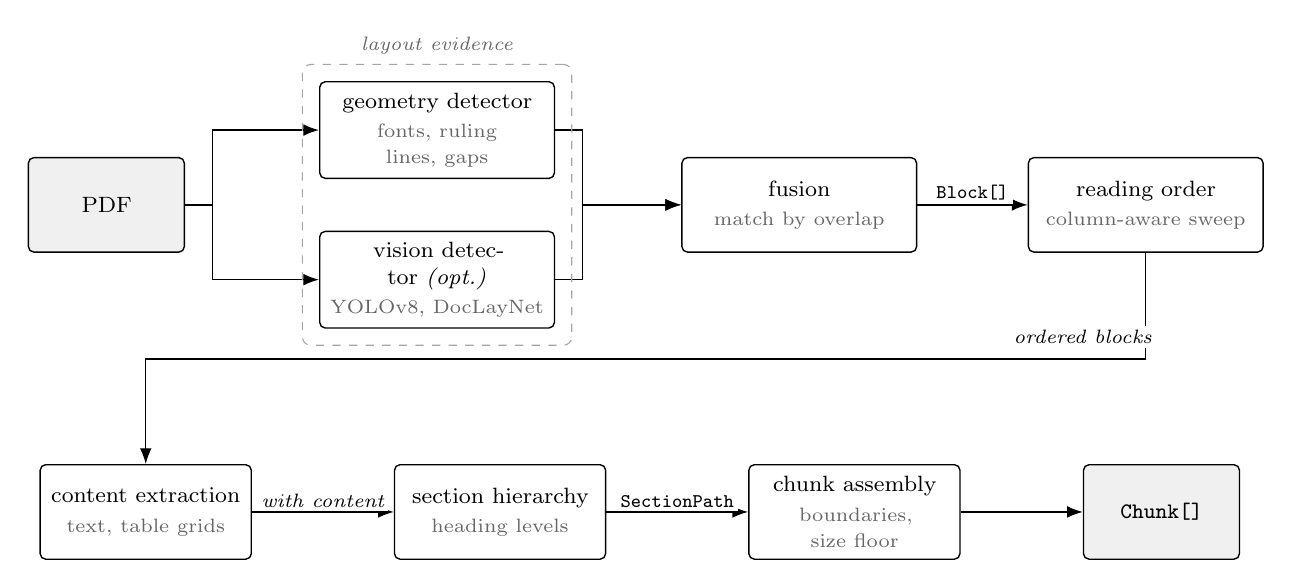
\begin{tikzpicture}[
 box/.style={draw, rounded corners=2pt, align=center, inner sep=4pt,
 minimum height=12mm, text width=27mm, line width=0.5pt,
 font=\footnotesize},
 term/.style={box, text width=17mm, fill=black!6},
 ar/.style={-{Latex[length=2mm]}, line width=0.5pt},
 lbl/.style={font=\scriptsize\itshape, inner sep=1.5pt, fill=white},
]
% --- row A: evidence and reconciliation
\node[term] (pdf) at (1.1, 0) {PDF};
\node[box]  (geo) at (5.3, 0.95) {geometry detector\\[1pt]{\scriptsize\color{black!60} fonts, ruling lines, gaps}};
\node[box]  (vis) at (5.3,-0.95) {vision detector \emph{(opt.)}\\[1pt]{\scriptsize\color{black!60} YOLOv8, DocLayNet}};
\node[box]  (fuse) at (9.9, 0) {fusion\\[1pt]{\scriptsize\color{black!60} match by overlap}};
\node[box]  (order) at (14.3, 0) {reading order\\[1pt]{\scriptsize\color{black!60} column-aware sweep}};

% --- row B: content and assembly
\node[box, text width=24mm] (extr) at (1.6, -3.9) {content extraction\\[1pt]{\scriptsize\color{black!60} text, table grids}};
\node[box, text width=24mm] (hier) at (6.1, -3.9) {section hierarchy\\[1pt]{\scriptsize\color{black!60} heading levels}};
\node[box, text width=24mm] (asm) at (10.6, -3.9) {chunk assembly\\[1pt]{\scriptsize\color{black!60} boundaries, size floor}};
\node[term] (out) at (14.5, -3.9) {\texttt{Chunk[]}};

\draw[ar] (pdf.east) -- ++(0.35,0) |- (geo.west);
\draw[ar] (pdf.east) -- ++(0.35,0) |- (vis.west);
\draw[ar] (geo.east) -- ++(0.35,0) |- (fuse.west);
\draw[ar] (vis.east) -- ++(0.35,0) |- (fuse.west);
\draw[ar] (fuse) -- node[lbl,above] {\upshape\texttt{Block[]}} (order);
\draw[ar] (order.south) -- ++(0,-1.35)
 node[lbl, above, pos=0.9, xshift=-8mm] {ordered blocks}
          -| (extr.north);
\draw[ar] (extr) -- node[lbl,above] {with content} (hier);
\draw[ar] (hier) -- node[lbl,above] {\upshape\texttt{SectionPath}} (asm);
\draw[ar] (asm)  -- (out);

\node[draw=black!35, dashed, rounded corners=3pt, inner sep=6pt,
 fit=(geo)(vis), label={[font=\scriptsize\itshape, color=black!60]above:layout evidence}]
      (evbox) {};
\end{tikzpicture}
\caption{The \ds{} pipeline. The two detectors read the same page through
disjoint evidence and never see each other's output; all reconciliation happens
in fusion. The label on each arrow names the object handed downstream, and each
stage receives a richer object than the one before it. Removing the vision
detector gives \dsg{}, which we report as its own system throughout. Only that
detector calls a model, and it is optional.}
\label{fig:pipeline}
\end{figure*}

\begin{figure*}[t]
\centering
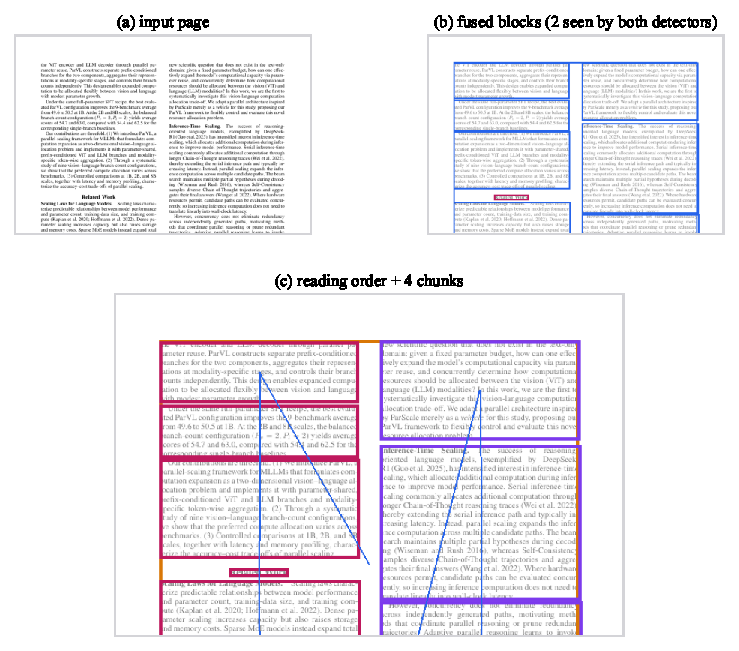
\includegraphics[width=0.90\textwidth]{pipeline.pdf}
\caption{The same path on a real page. (a) the input page as the PDF stores it;
(b) the blocks after fusion, coloured by type, with the count both detectors
agreed on; (c) the reading order the pipeline infers, drawn as a line through
the block centres, and the four chunks it cuts.}
\label{fig:realpage}
\end{figure*}

\ds{} represents each chunk as a structured object containing its text, page number, reading-order position, block type, source block identifiers, and section path. The section path records the hierarchy of headings associated with the chunk. This structural information is preserved alongside the text and can therefore be used by downstream retrieval. Figure~\ref{fig:pipeline} shows the stages of the pipeline, and Figure~\ref{fig:realpage} shows the same path applied to a real page.

\subsection{Finding the Blocks}
\label{sec:detect}

\ds{} uses two complementary block detectors. The first is geometry-based and operates directly on PDF primitives, including text positions, font properties, ruling lines, and whitespace. These signals are used to group text into lines and blocks and to identify structural elements such as headings, tables, figures, and captions.

The second detector is a YOLOv8 model trained on DocLayNet \citep{pfitzmann2022doclaynet}. It operates on a rendered image of each page and independently proposes regions based on visual appearance. The two detectors therefore provide complementary views of the page: geometry captures information explicitly available in the PDF, while vision can identify structures that leave little or no geometric trace, such as borderless tables.

\subsection{Fusion and Reading Order}
\label{sec:fusion}

The two sets of detected regions are reconciled using bounding-box overlap. Matching regions are merged, while regions detected by only one detector are retained. This allows, for example, a borderless table identified by the vision detector to survive even when the geometry-based detector cannot detect it.

The resulting blocks are then ordered by page layout. For pages with multiple columns, \ds{} identifies column bands from horizontal gaps between blocks and reads each band from top to bottom. Captions are associated with nearby figures or tables. Page-level orders are then combined into a document-wide reading order.

\subsection{Extracting Text and Tables}
\label{sec:extract}

Once the blocks have been identified and ordered, their contents are extracted using \texttt{pdfplumber}. Text extraction uses a font-size-aware word-spacing tolerance to reduce cases where closely spaced words are incorrectly merged.

Tables are extracted as grids when ruling lines provide sufficient structure. When the grid representation covers only part of a table, \ds{} falls back to the raw text of the whole region, so the unruled rows are kept. The resulting table text is used for retrieval, while a separate Markdown representation can be generated for structured presentation.

\subsection{Reconstructing the Outline and Chunking}
\label{sec:chunking}

\ds{} reconstructs the document hierarchy from detected headings. Heading levels are inferred from explicit numbering when available and otherwise from relative font size, with the hierarchy limited to three levels. Each non-heading block inherits the headings above it as its section path.

Chunks are then assembled in reading order. Headings normally close the current text buffer and update the active section path, while body text accumulates up to a 500-word limit with a 75-word carry-over. Tables are kept as independent chunks, captions remain associated with their figures, and the reference list is excluded.

To avoid producing short chunks around headings, a heading does not close the current buffer until it contains at least 200 words. Chunk sizes are counted in whitespace-separated words, so boundaries do not depend on a tokenizer version. Parsed blocks are cached under a content hash, so a change to chunking parameters reruns only this last stage.

% =====================================================================
\section{Experimental Setup}
\label{sec:setup}

We evaluate \ds{} against five existing chunking approaches: PyMuPDF4LLM, Unstructured, LangChain's recursive splitter, LlamaIndex's sentence splitter, and LlamaIndex's semantic splitter. We also report our own geometry-only variant, \dsg{}, as a separate system, giving seven systems in total. All systems are evaluated through the same retrieval harness, so only the chunking method varies. Chunks are indexed using both BM25 \citep{robertson2009bm25} and embeddings from \texttt{all-MiniLM-L6-v2} \citep{reimers2019sbert}, with the rankings combined using reciprocal rank fusion at $k{=}60$ \citep{cormack2009rrf}. The retriever returns the top five chunks per question, and performance is measured using mean reciprocal rank (MRR) with bootstrap confidence intervals and paired bootstrap significance tests \citep{efron1993bootstrap}. Two baselines are absent. LumberChunker \citep{duarte2024lumberchunker} calls a language model for every document, which our compute budget did not cover; LlamaIndex's semantic splitter is the only model-based chunker we compare. Docling \citep{auer2024docling}, the closest layout-aware baseline, has an adapter in our harness but never completed a run on our hardware.

We use three complementary datasets. OHR-Bench \citep{zhang2025ocrhindersrag} provides the primary retrieval evaluation, containing 95 born-digital documents and 3{,}558 human-written questions with annotated evidence. For structural evaluation, we use 134 papers from PubMed Central together with their publisher-provided JATS XML, fetched through Europe PMC \citep{europepmc}, allowing chunk boundaries to be compared against the original section structure without involving a retriever. FinanceBench \citep{islam2023financebench} is evaluated separately to determine whether the retrieval protocol is suitable for financial question answering (\S\ref{sec:financebench}).

Retrieval relevance is measured using three criteria. Under the \textbf{span} rule, a chunk is relevant if it contains the gold answer sentence. Under the \textbf{region} rule, it is relevant if its overlap coefficient with the annotated evidence (shared words over the smaller of the two) is at least $0.7$, a value we fixed before scoring any system. Under the \textbf{page} rule, it is relevant if it comes from the annotated page. All three rules are applied to the same retrieved chunks, allowing the effect of the relevance definition itself to be isolated.

We additionally evaluate structural recovery using Pk \citep{beeferman1999statistical} and WindowDiff \citep{pevzner2002critique}, and test reproducibility by processing the OHR-Bench documents twice in separate processes and comparing the resulting chunk identifiers, metadata, and content.

% =====================================================================
\section{Results and Analysis}
\label{sec:results}

\subsection{Retrieval Performance and Relevance Criteria}
\label{sec:inversion}

\begin{table}[t]
\centering
\small
\caption{OHR-Bench: 95 documents, 3{,}558 human-written questions, seven
chunkers, MRR under three relevance rules on \emph{identical chunks}. Rank in
parentheses; best MRR per rule in bold. Ctx is the number of context words
returned per query (top five chunks).}
\label{tab:ohr}
\setlength{\tabcolsep}{3pt}
\begin{tabular}{@{}lcccr@{}}
\toprule
System & page & span & region & ctx \\
\midrule
\ds{}            & 0.600 (6) & \best{0.706 (1)} & \best{0.666 (1)} & 2194 \\
\dsg{}           & 0.470 (7) & 0.705 (2) & 0.657 (2) & 2328 \\
PyMuPDF4LLM      & 0.668 (4) & 0.699 (3) & 0.604 (3) & 2424 \\
Unstructured     & \best{0.795 (1)} & 0.654 (5) & 0.601 (5) & 560 \\
LangChain        & 0.756 (2) & 0.641 (7) & 0.603 (4) & 638 \\
LlamaIndex       & 0.729 (3) & 0.648 (6) & 0.589 (6) & 1430 \\
LlamaIndex-sem   & 0.652 (5) & 0.654 (4) & 0.575 (7) & 4698 \\
\bottomrule
\end{tabular}
\end{table}

\begin{figure}[t]
\centering
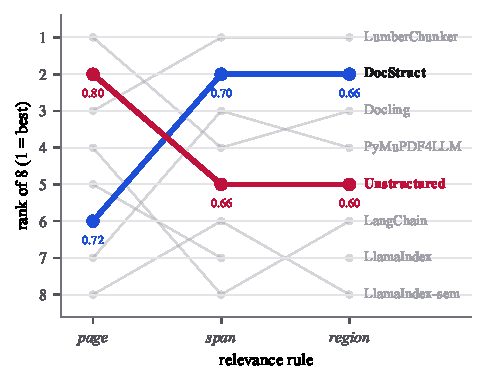
\includegraphics[width=\columnwidth]{mode_inversion.pdf}
\caption{Rank under each relevance rule, same chunks throughout. \ds{} runs
6th, 1st, 1st and \texttt{unstructured} runs 1st, 5th, 5th. The only thing that
changes between the columns is the rule that decides whether a retrieved chunk
counts.}
\label{fig:inversion}
\end{figure}

The choice of relevance criterion substantially changes the chunker leaderboard (Table~\ref{tab:ohr}, Figure~\ref{fig:inversion}). \ds{} ranks first under both the span and region rules but sixth under the page rule, while Unstructured shows the opposite pattern. Under the region rule, \ds{} significantly outperforms every external system; under span, it significantly outperforms four of the five external systems, with PyMuPDF4LLM statistically indistinguishable from it ($p=0.23$). Under page, \ds{} is outperformed by four systems.

The reversal tracks chunk size. \ds{} returns 2{,}194 context words per query and Unstructured 560, and a larger chunk contains more answer sentences, so the span rule rewards size directly. Our span lead could therefore come from context volume alone, and under span the top three systems sit within $0.007$ MRR of each other. The region rule normalises overlap by the smaller side and should not reward size. Across the seven systems, the Spearman correlation between mean chunk width and MRR is $+0.571$ under span, $-0.679$ under page and $+0.036$ under region ($n{=}7$; no correlation reaches $p<0.05$), so region shows no size trend in our data and is the rule our claim rests on. We tested this directly by raising each small-chunk system's top-$k$ until its context matched that of \dsg{} at $k{=}5$ (2{,}328 words): Unstructured at $k{=}20$ (2{,}193 words), LangChain at $k{=}17$ (2{,}137) and LlamaIndex at $k{=}8$ (2{,}264), all on one install whose $k{=}5$ runs reproduce Table~\ref{tab:ohr} within $0.003$ MRR. \dsg{} still leads every one of them, by $0.043$ to $0.060$ MRR under span and $0.047$ to $0.064$ under region, with every paired 95\% interval above zero. A larger $k$ moves MRR little, since a hit below rank five adds at most $1/6$; recall is where the budget shows, and under span Unstructured at $k{=}20$ recalls $0.800$ of answers against $0.789$ for \dsg{}. Within the \ds{} variants, the page-rule gap ($0.600$ against $0.470$) follows chunk count, 9{,}080 against 5{,}810.

\begin{figure}[t]
\centering
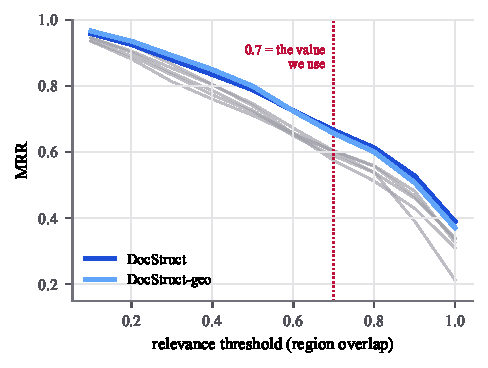
\includegraphics[width=\columnwidth]{threshold_sweep.pdf}
\caption{Region relevance re-scored on one run as the overlap threshold moves
from $0.1$ to $1.0$. The \ds{} family leads at every setting; which member of
the family leads does not. Below $0.6$ it is \dsg{}.}
\label{fig:sweep}
\end{figure}

The $0.7$ threshold predates every score in this paper, but it also happens to be where our margin over the field peaks, so we sweep it from $0.1$ to $1.0$ on the same retrieved results (Figure~\ref{fig:sweep}). One of the two \ds{} variants leads at every value, with a margin of $0.045$ or more over the best external system from $0.4$ up. Which variant leads changes: \dsg{} leads below $0.6$, so the hybrid's first place in Table~\ref{tab:ohr} holds only for strict thresholds.

The aggregate retrieval advantage is strongest on law and manuals. \ds{} trails Unstructured on academic papers and LlamaIndex's semantic splitter on finance, and performs below the best external system on questions whose evidence is contained in tables, where the best external score is $0.307$ against our $0.288$. These results suggest that chunk size and document type both influence retrieval performance.

\subsection{Structural Recovery}
\label{sec:sections}

\begin{table}[t]
\centering
\small
\caption{Section-boundary agreement with publisher-written JATS gold on 134
PubMed Central papers. Pk and WindowDiff are error rates; lower is better.
Unstructured covers 99 documents because it hard-failed on 35.}
\label{tab:sections}
\begin{tabular}{@{}lccr@{}}
\toprule
System & WinDiff & Pk & Chunks/doc \\
\midrule
\dsg{}            & \best{0.423} & \best{0.342} & 26.8 \\
PyMuPDF4LLM       & 0.480 & 0.449 & 17.7 \\
\ds{}             & 0.482 & 0.353 & 37.5 \\
LlamaIndex-sem    & 0.534 & 0.513 & 29.1 \\
LlamaIndex        & 0.695 & 0.598 & 42.7 \\
LangChain         & 0.879 & 0.620 & 85.6 \\
Unstructured$^{*}$ & 0.893 & 0.603 & 106.9 \\
\bottomrule
\multicolumn{4}{@{}l@{}}{\scriptsize $^{*}$ 99 of 134 documents; 35 hard failures.} \\
\end{tabular}
\end{table}

\begin{figure}[t]
\centering
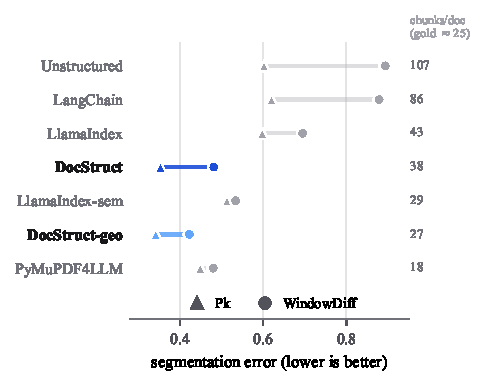
\includegraphics[width=\columnwidth]{size_confound.pdf}
\caption{Table~\ref{tab:sections} as a picture. Triangles are Pk, dots are
WindowDiff; the right margin gives chunks per document against roughly 25 real
sections. The two tools that cut most are last under one metric and mid-table
under the other.}
\label{fig:sections}
\end{figure}

To evaluate structure independently of retrieval, we compare each chunker's boundaries with the section boundaries recorded in the publisher-provided JATS XML. \dsg{} achieves the best scores on both Pk and WindowDiff (Table~\ref{tab:sections}, Figure~\ref{fig:sections}), ahead of our own hybrid at $2.4\times$ the speed. This provides evidence that the layout-based pipeline can recover document structure without relying on retrieval performance.

The metric and the design do not fully match: $57.4\%$ of the gold sections are shorter than \ds{}'s 200-word minimum, so \ds{} merges them by construction and the score partly measures how the floor treats short sections. Agreement with publisher sections also measures structural recovery, and says nothing about whether those boundaries suit retrieval.

\subsection{Reproducibility}
\label{sec:determinism}

We parse all 95 OHR-Bench documents twice in independent processes with the geometry-only pipeline and compare every chunk's identifier, type, page, reading-order position, section path and content. All 5{,}810 chunks are byte-identical. The claim covers one code version and the geometry-only path; the hybrid runs GPU inference, which this test does not cover.

\subsection{Failure Analysis}
\label{sec:cost}

The vision detector does not produce a measurable retrieval improvement on OHR-Bench: adding it changes MRR by only $+0.0012$ under span ($p=0.80$) and $+0.0090$ under region ($p=0.12$). Geometry-only scores better on section boundaries and runs faster. The one place it changes the output is borderless tables: on a single SEC filing (3M's 2018 10-K) it finds 122 tables where geometry finds 4. That is a detection count, and testing whether it helps retrieval needs a table-heavy corpus whose questions our retriever can reach. Until one shows a gain, we recommend \dsg{} as the default.

\ds{} also uses substantially more retrieval context than the smallest baseline. It produces approximately 2{,}194 context words per query compared with 560 for Unstructured, a $3.9\times$ larger context bill. Its word coverage is $0.9632$ compared with $1.000$ for LangChain, while its duplication rate is $1.83\times$, the highest of the seven systems compared.

Finally, we do not report a FinanceBench leaderboard.
\label{sec:financebench}
A pilot on two 10-K filings and seven questions scored MRR $0$ for both systems we ran. We checked the harness first. Each question has a chunk whose region overlap with the evidence is $0.990$ or $1.000$, and the retriever does rank it, at positions 42 to 299 under three different encoders, so the scoring works and the evidence sits outside the top five. The questions are analyst prompts with little word overlap with their evidence, the evidence is a numeric table, and one filing yields 729 to 1{,}176 chunks. \citet{elbachyr2026empirical} reach MRR $0.700$--$0.844$ on these filings with a different retriever and page-level gold. The same weakness appears on OHR-Bench as table-sourced questions, where every system scores between $0.19$ and $0.31$ span MRR and only $35.7\%$ of the table evidence appears in the raw text at all. Two untested changes target it: header--value serialisation of table rows, implemented behind a default-off flag, and the vision detector's borderless-table proposals.

% =====================================================================
\section{Conclusion}
\label{sec:conclusion}

\ds{} recovers layout before chunking and produces deterministic chunks with no language model on the parsing path. It ranks first under two of three relevance rules, leads on publisher section boundaries, and reproduces byte for byte. Its vision component adds no measurable retrieval gain, and it spends about four times the context of the leanest baseline.

The broader finding is about evaluation itself: chunker rankings depend on how relevance is defined, and no relevance rule is neutral to chunk size. The same chunks rank differently under reasonable criteria, so chunking comparisons should state their relevance rule and evaluate under more than one.

% =====================================================================
\section*{Limitations}
\label{sec:limitations}

\paragraph{Scope.} \ds{} reads the PDF text layer and performs no OCR, which keeps it deterministic; scanned PDFs without a text layer are out of scope, and every baseline also runs with OCR off. All corpora are English. Two parts of the pipeline assume a space-delimited Latin script: chunk sizes count whitespace-separated words, and heading levels read Arabic, Roman and appendix numbering. Neither has been tested on other scripts, and a language without spaces between words would break the size floor. The reading-order heuristic handles at most two columns and can misplace full-width elements above a two-column body.

\paragraph{Context budget and baselines.} At $k{=}5$ \ds{} returns about four times more context per query than Unstructured. Matching the budget by raising the baselines' top-$k$ leaves our MRR lead in place (\S\ref{sec:inversion}), but that run covers \dsg{} and not the hybrid, omits the page rule, and does not try the other remedy, resizing the baselines' chunks. LumberChunker and Docling are missing for the reasons in \S\ref{sec:setup}.

\paragraph{Parse fidelity.} We do not evaluate PDF parsing fidelity with benchmarks such as OmniDocBench or READoc; our structural evaluation instead measures agreement with publisher-provided section boundaries. We report no layout detection accuracy: our two annotated documents were drafted from the pipeline's output, so a score would favour \ds{}, and DocLayNet is the vision detector's training data. The detector-fusion weights remain unvalidated (\S\ref{sec:fusion}).

\paragraph{Chunking and fusion parameters.} The 200-word minimum and 500-word maximum were chosen on an internal corpus whose annotations we later found unreliable, and we exclude its results. No benchmark in this paper has tuned or ablated them, and the fusion overlap threshold has not been ablated either.

\paragraph{Computational cost.} Three long financial filings exceeded the 30-minute parse limit in the determinism evaluation.

% =====================================================================
\section*{Ethics Statement}

All three corpora are public and are fetched by script instead of redistributed. None involves human subjects or personal data beyond published author lists. The parse pipeline calls no language model, so its cost is local CPU time; the only model use in the project is a vision detector that the results show can be switched off. We report our losses in the main text.

% =====================================================================
\section*{Acknowledgements}

I thank the SFI Data team for the opportunity to work in document intelligence, and I am especially grateful to Anirudh Valluri and Michael Susan for their guidance and collaboration.

% =====================================================================
\bibliographystyle{acl_natbib}
\bibliography{refs}

\end{document}
